%!TEX root =  main.tex
\section{Experimental Results}
\label{sec:results}
% Valid test: uniformity of p-vals, good sigma estimate, and unequal group sizes.
% We assess performance using power. talk through power incontext of different eps.
% optimal rho
% Last bit: comparison to campbell

In this section we assess the properties and performance of Algorithm~\ref{alg:pval} through simulation. 

\subsection{Properties of the test}\label{subsec:properties}

A $p$-value is considered valid if ~\cite{casellaberger2002}

$$
\Pr[p\textrm{-value} \le \alpha \mid \X \leftarrow H_0] \le \alpha.
$$

In other words, the actual type I error rate must be less than or equal to $\alpha$. This can be assessed by conducting many tests on simulated data sampled according to $H_0$ at various $\alpha$ and checking if the proportion of rejections is less than or equal to $\alpha$. 

Figure~\ref{Fig:valid-pvals} presents these simulations for several choices of $\epsilon$ and demonstrates that the $F_1$ test produces valid $p$-values. The type I error rate is lowest at low $\epsilon$ values because the high privacy guarantee requires a large amount of noise be added to \se, which can lead to a negative estimate for $\sigma$, which in turns leads to an automatic decision to retain $H_0$ (see section~\ref{subsec:alg-method}).

\begin{figure}
\centering
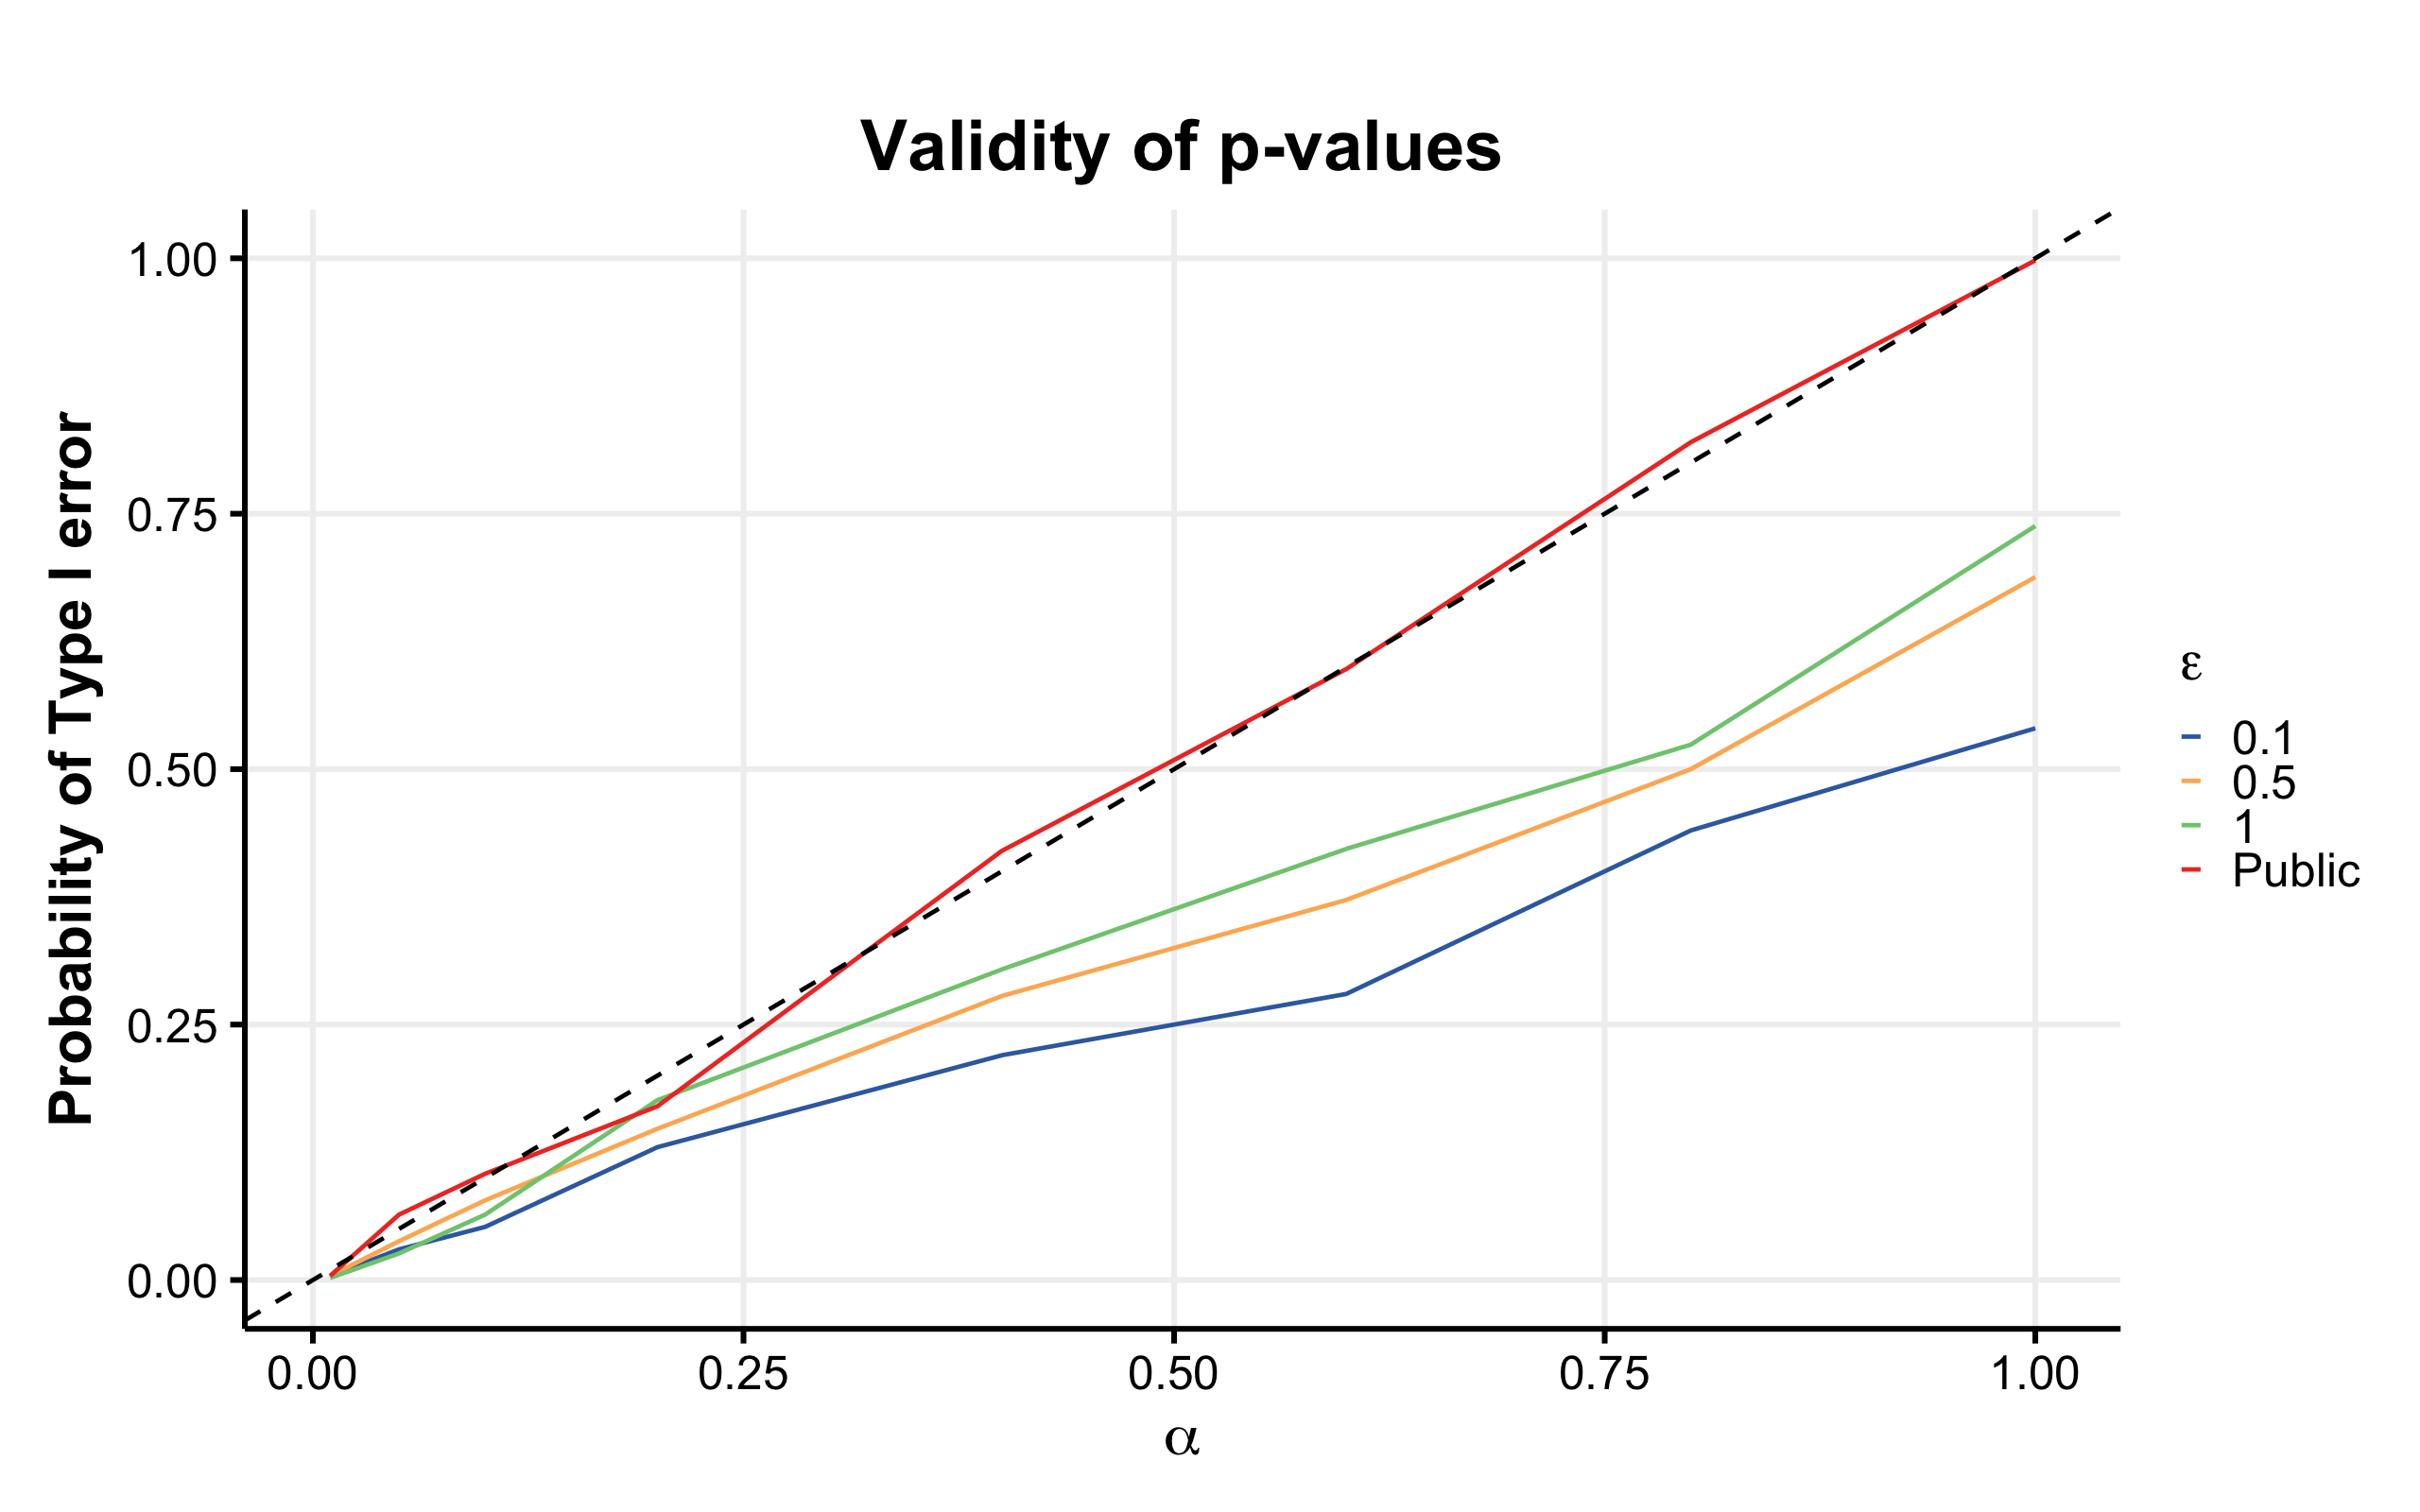
\includegraphics[width=.8\linewidth]{valid-pvals.png}
\caption{The empirical type I error rate under three private scenarios is less than $\alpha$ while the public error rate is exactly $\alpha$ (within MC variability). Each point in a line represents 500 simulated tests, each with $N = 180$, $k=3$, and equal-size groups.\label{Fig:valid-pvals}}
\end{figure}

We note also that when we simulate data for calculating a reference distribution, we always simulate data with equal-size groups.  I.e., we must confirm that the critical value of the reference distribution is highest when groups are of equal size.  Fortunately, this appears to be the case.  Appendix \ref{app:unequal} contains both experimental and theoretical arguments for this claim, though not a complete analytic proof.

% \subsection{Varying the $\epsilon$ allocation}
% In Algorith~\ref{alg:F1}, we divide the epsilon budget equally between the numerator and denominator of the statistics by allocating $\epsilon/2$ to each of \sa and \se. This is a perfectly reasonable starting point. We wondered if allocating more of the epsilon budget to the \sa would improve the power of the statistic, since we use $\sa/(\dbsize - \k)$ as our standard deviation estimate\ab{I thought we used SE/N?}. This modifies our algorithm slightly; rather than allocating \eps/2 to each of \sa and \se, we will allocate a portion $\epsfrac \cdot \eps$ to the \sa  computation, and $(1-\epsfrac)\cdot \eps$ to the \se computation, where $\epsfrac \in [0,1]$.  In other words, \epsfrac is the proportion of our epsilon budget that we will allocate to the \sa computation. This proportion could potentially be user-defined, but we found a particular value for \epsfrac to be superior, so it will be a constant. We used the same method for calculating the $p$-value for a statistic as the regular $F_1$ (Algorithm~\ref{alg:pval}).
% 
% Our updated algorithm is as follows: \ms{Not sure if it's clear enough to just describe or if we want to have the full algorithm. I put it in here so we can decide later}
% \begin{algorithm}
%     \caption{Differentially private ANOVA with Absolute Values and varying Epsilon Allocation \label{alg:F1epsfrac}}
%     \begin{algorithmic}
%         \STATE \textbf{Input:} Database $\x$, $\eps$ value, epsilon allocation $\epsfrac \in (0,1)$
%         \STATE Compute $\widehat{\sa} = \sa(x) + Z_1$ where $Z_1\sim\text{Lap}\left(\frac{4}{\eps\cdot\epsfrac}\right)$
%         \STATE Compute $\widehat{\se} = \se(x) + Z_2$ where $Z_2\sim\text{Lap}\left(\frac{3}{\eps\cdot(1-\epsfrac)}\right)$
%         \STATE Compute $\widehat{F_1} = \frac{\widehat{\sa}/(k-1)}{\widehat{\se}/(n-k)}$
%         \STATE \textbf{Output:} $\widehat{F_1}, \widehat{\sa}, \widehat{\se}$
%     \end{algorithmic}
% \end{algorithm}
% 
% \begin{theorem}
% Algorithm~\ref{alg:F1epsfrac} is \eps -differentially private.
% \end{theorem}
% \begin{proof}
% As before, we use the Laplace Mechanism (Definition~\ref{thm:lapmechanism}) to compute the \sa and \se with privacy $\eps\cdot\epsfrac$ and $\eps\cdot(1-\epsfrac)$, respectively. Since the number of groups \k and total database size \dbsize are public information, computing $\widehat{F_1}$ is post-processing (Theorem~\ref{thm:postprocessing}) and does not affect the privacy of Algorithm~\ref{alg:F1epsfrac} . Thus, by the composition theorem (Theorem~\ref{thm:composition}), Algorithm~\ref{alg:F1epsfrac} is $\eps\cdot\epsfrac + \eps\cdot(1-\epsfrac) = \eps$-differentially private.
% \end{proof}

\subsection{Optimal \epsfrac}\label{subsec:optrho}

The computation of the private $F_1$ statistic requires the specification of $\epsfrac \in (0, 1)$, the parameter that determines the proportion of the privacy budget that is allocated to \sa relative to \se. We determined an optimal value for $\epsfrac$ by constructing power plots comparing database size to power for different \epsfrac values. We began by exploring the full range from $0.1$ to $0.9$ by $0.1$-increments to get a sense of the range of variability in power. After that initial pass, we tuned in to the value with higher precision. We considered many effect sizes and found that in every case $\epsfrac \approx 0.7$ was the most powerful.

Figure~\ref{Fig:f1-epsfrac} is an example of one of the many scenarios that were considered, which identifies .7 as the optimal value. The scale of the effect of $\rho$ on power is not dramatic but it was persistent across scenarios.

% We hypothesize that this difference comes from  either the difference in sensitivities of \sa and \se, or that having an accurate numerator contributes more to the overall accuracy of the statistic (?). \ms{Someone find an intelligent justification for this} \ar{Any justification will need to be backed up with a result -- think about how you could test this hypothesis.  If it remains speculative, it should go in the Discussion/Conclusion section, not in Results.}  Since we are not able to compute the optimal \epsfrac analytically, we resort to simulation across many effect sizes and database sizes to find the best \epsfrac.

\begin{figure}
\centering
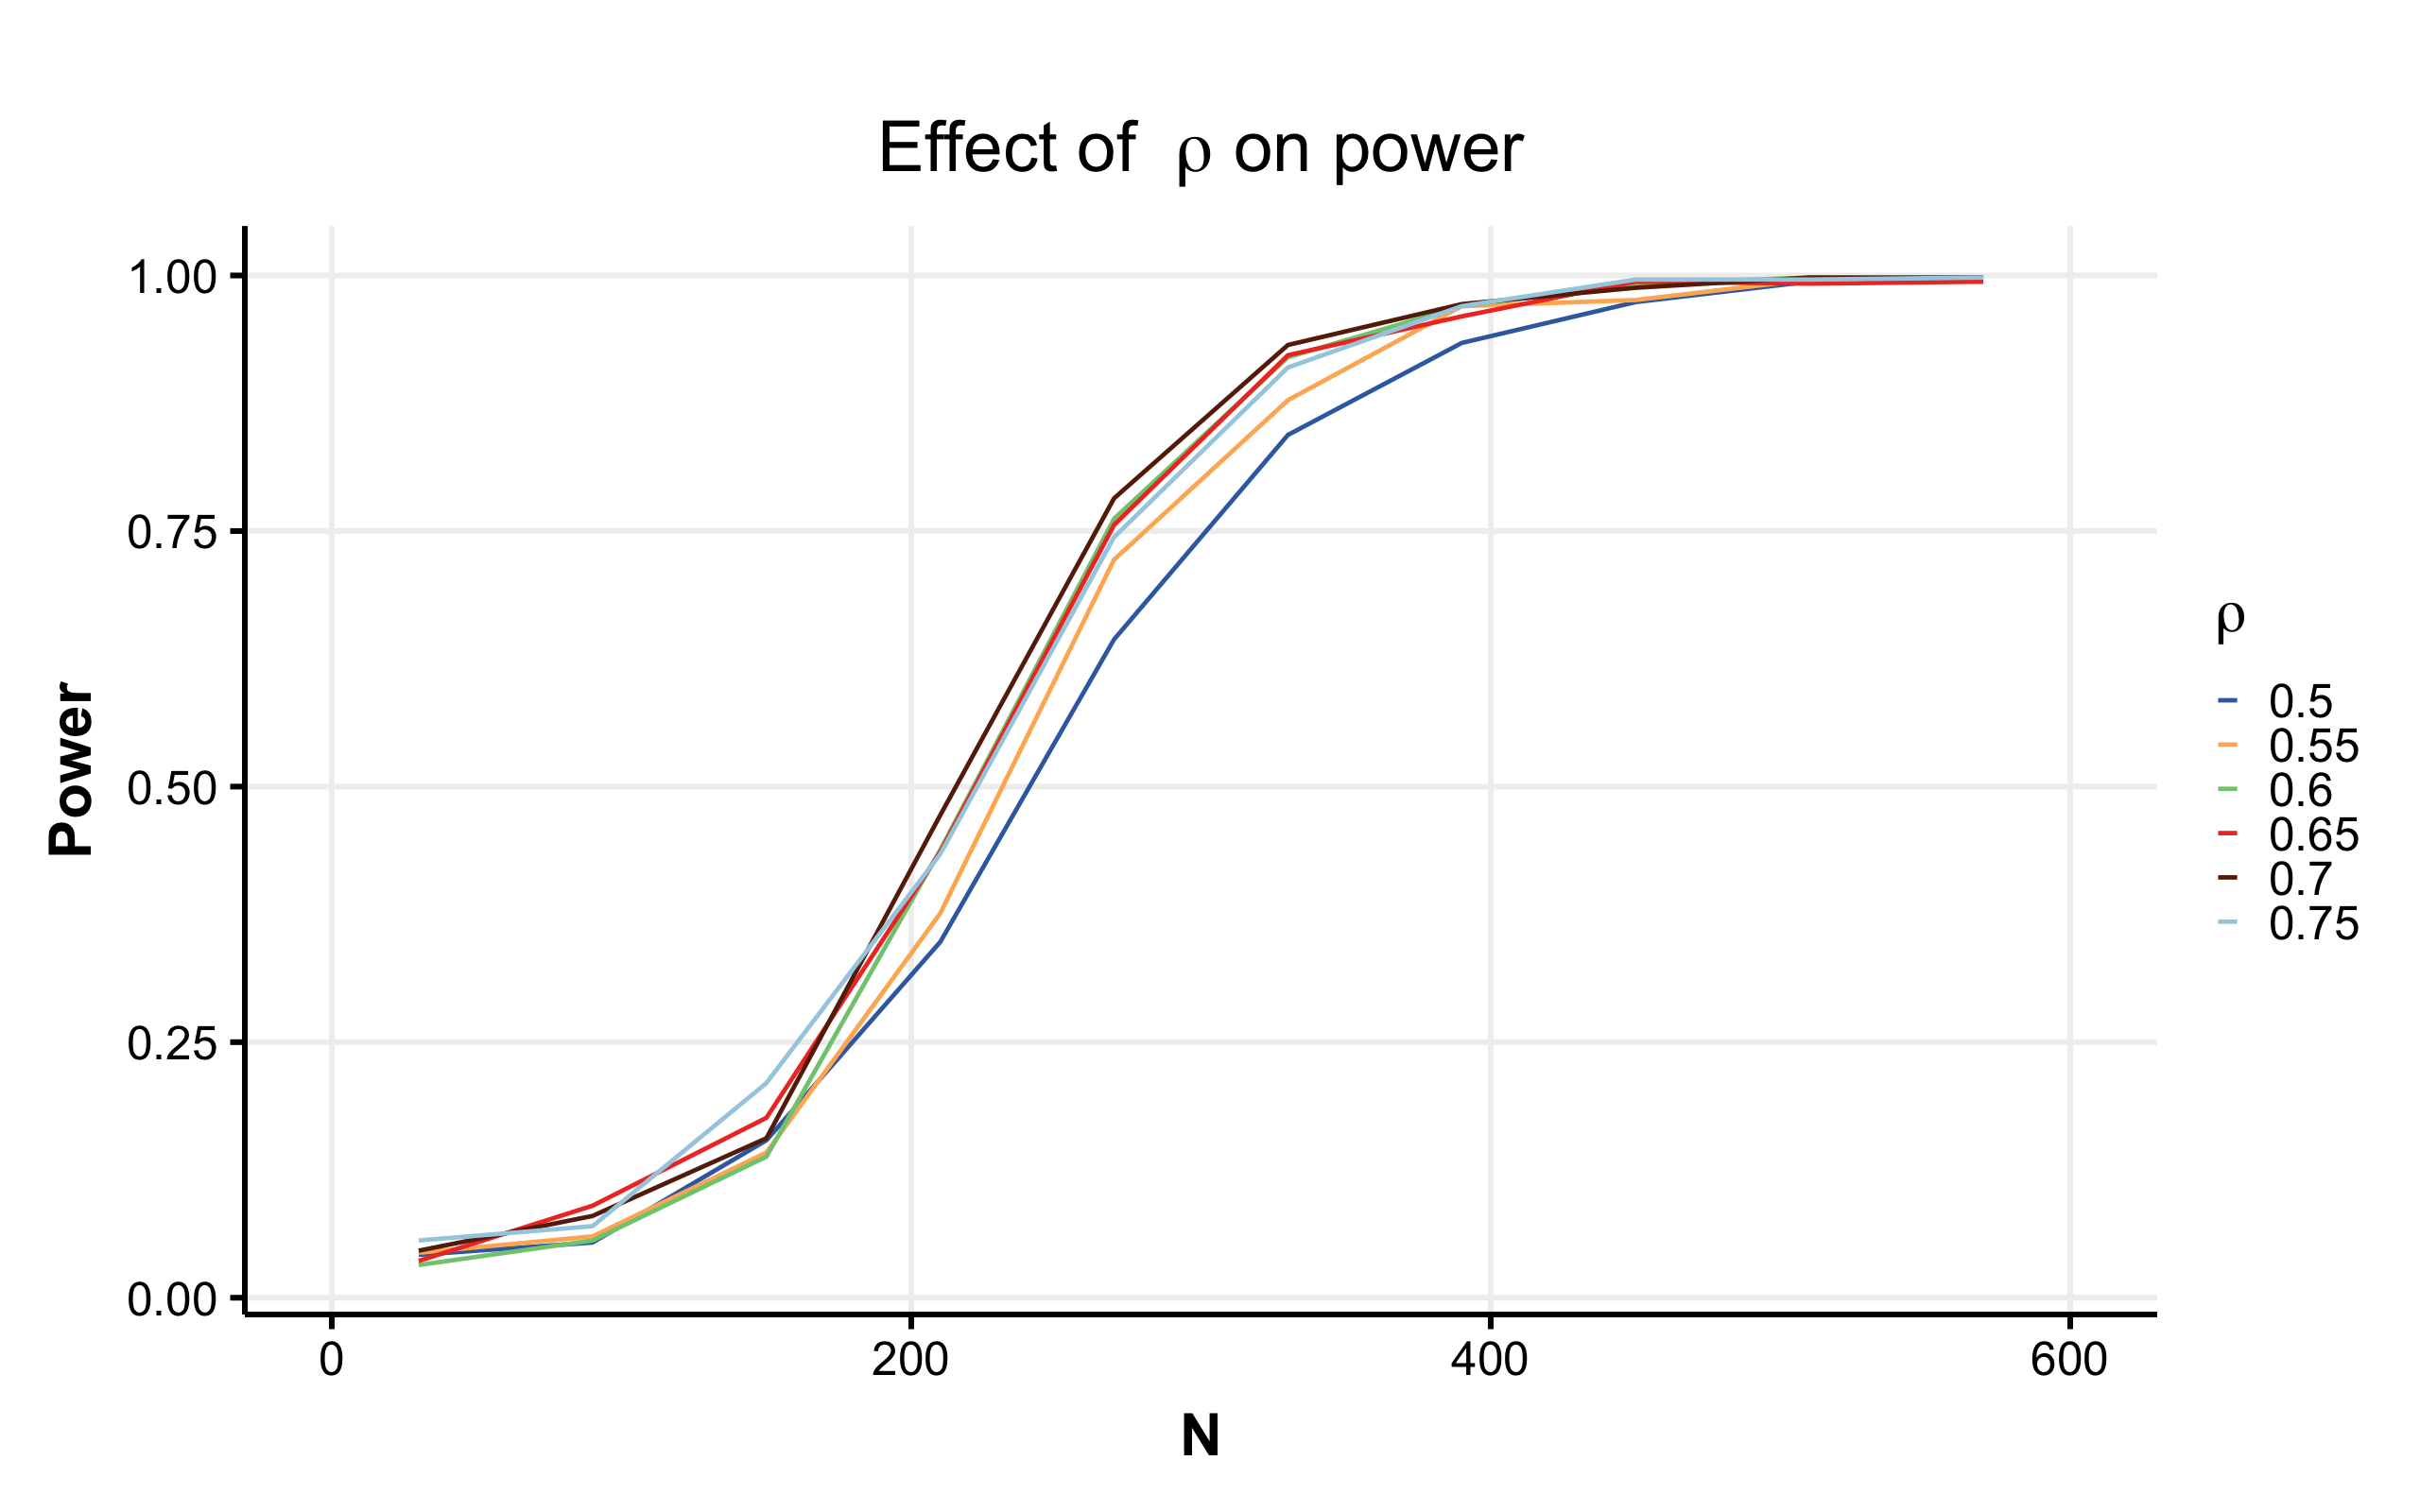
\includegraphics[width=.6\linewidth]{f1-epsfrac.png}
\caption{Power curves at varying $\rho$ in a setting where $\epsilon = 1$, $k = 3$, $\sigma = .15$, and effect size: $1\sigma$. Power is experimentally maximized when $\rho = .7$.\label{Fig:f1-epsfrac}}
\end{figure}

\subsection{Performance of the test: power}
\label{subsec:power-analysis}

There can be many tests for a given scientific setting that generate valid $p$-values and have identical type I error rates. What distinguishes them is their statistical power, or the probability that they reject $H_0$ when the database comes from a distribution under $H_A$.

The most common way to assess the power of a test is to generate a plot of power as a function either of database size or of effect size. Figure~\ref{Fig:f1} fixes the effect size and shows power curves as a function of database size for four choices of $\epsilon$. An ideal test would very quickly develop power near 1 with very little data. In our private setting, it is clear that the cost of high privacy ($\epsilon = .1$) is roughly an order of magnitude more data than modest privacy ($\epsilon = 1$) to achieve high power. Our private test (for reasonable values of $\epsilon$) still requires much more data than the public version, hundreds of data points as opposed to dozens.

\begin{figure}
\centering
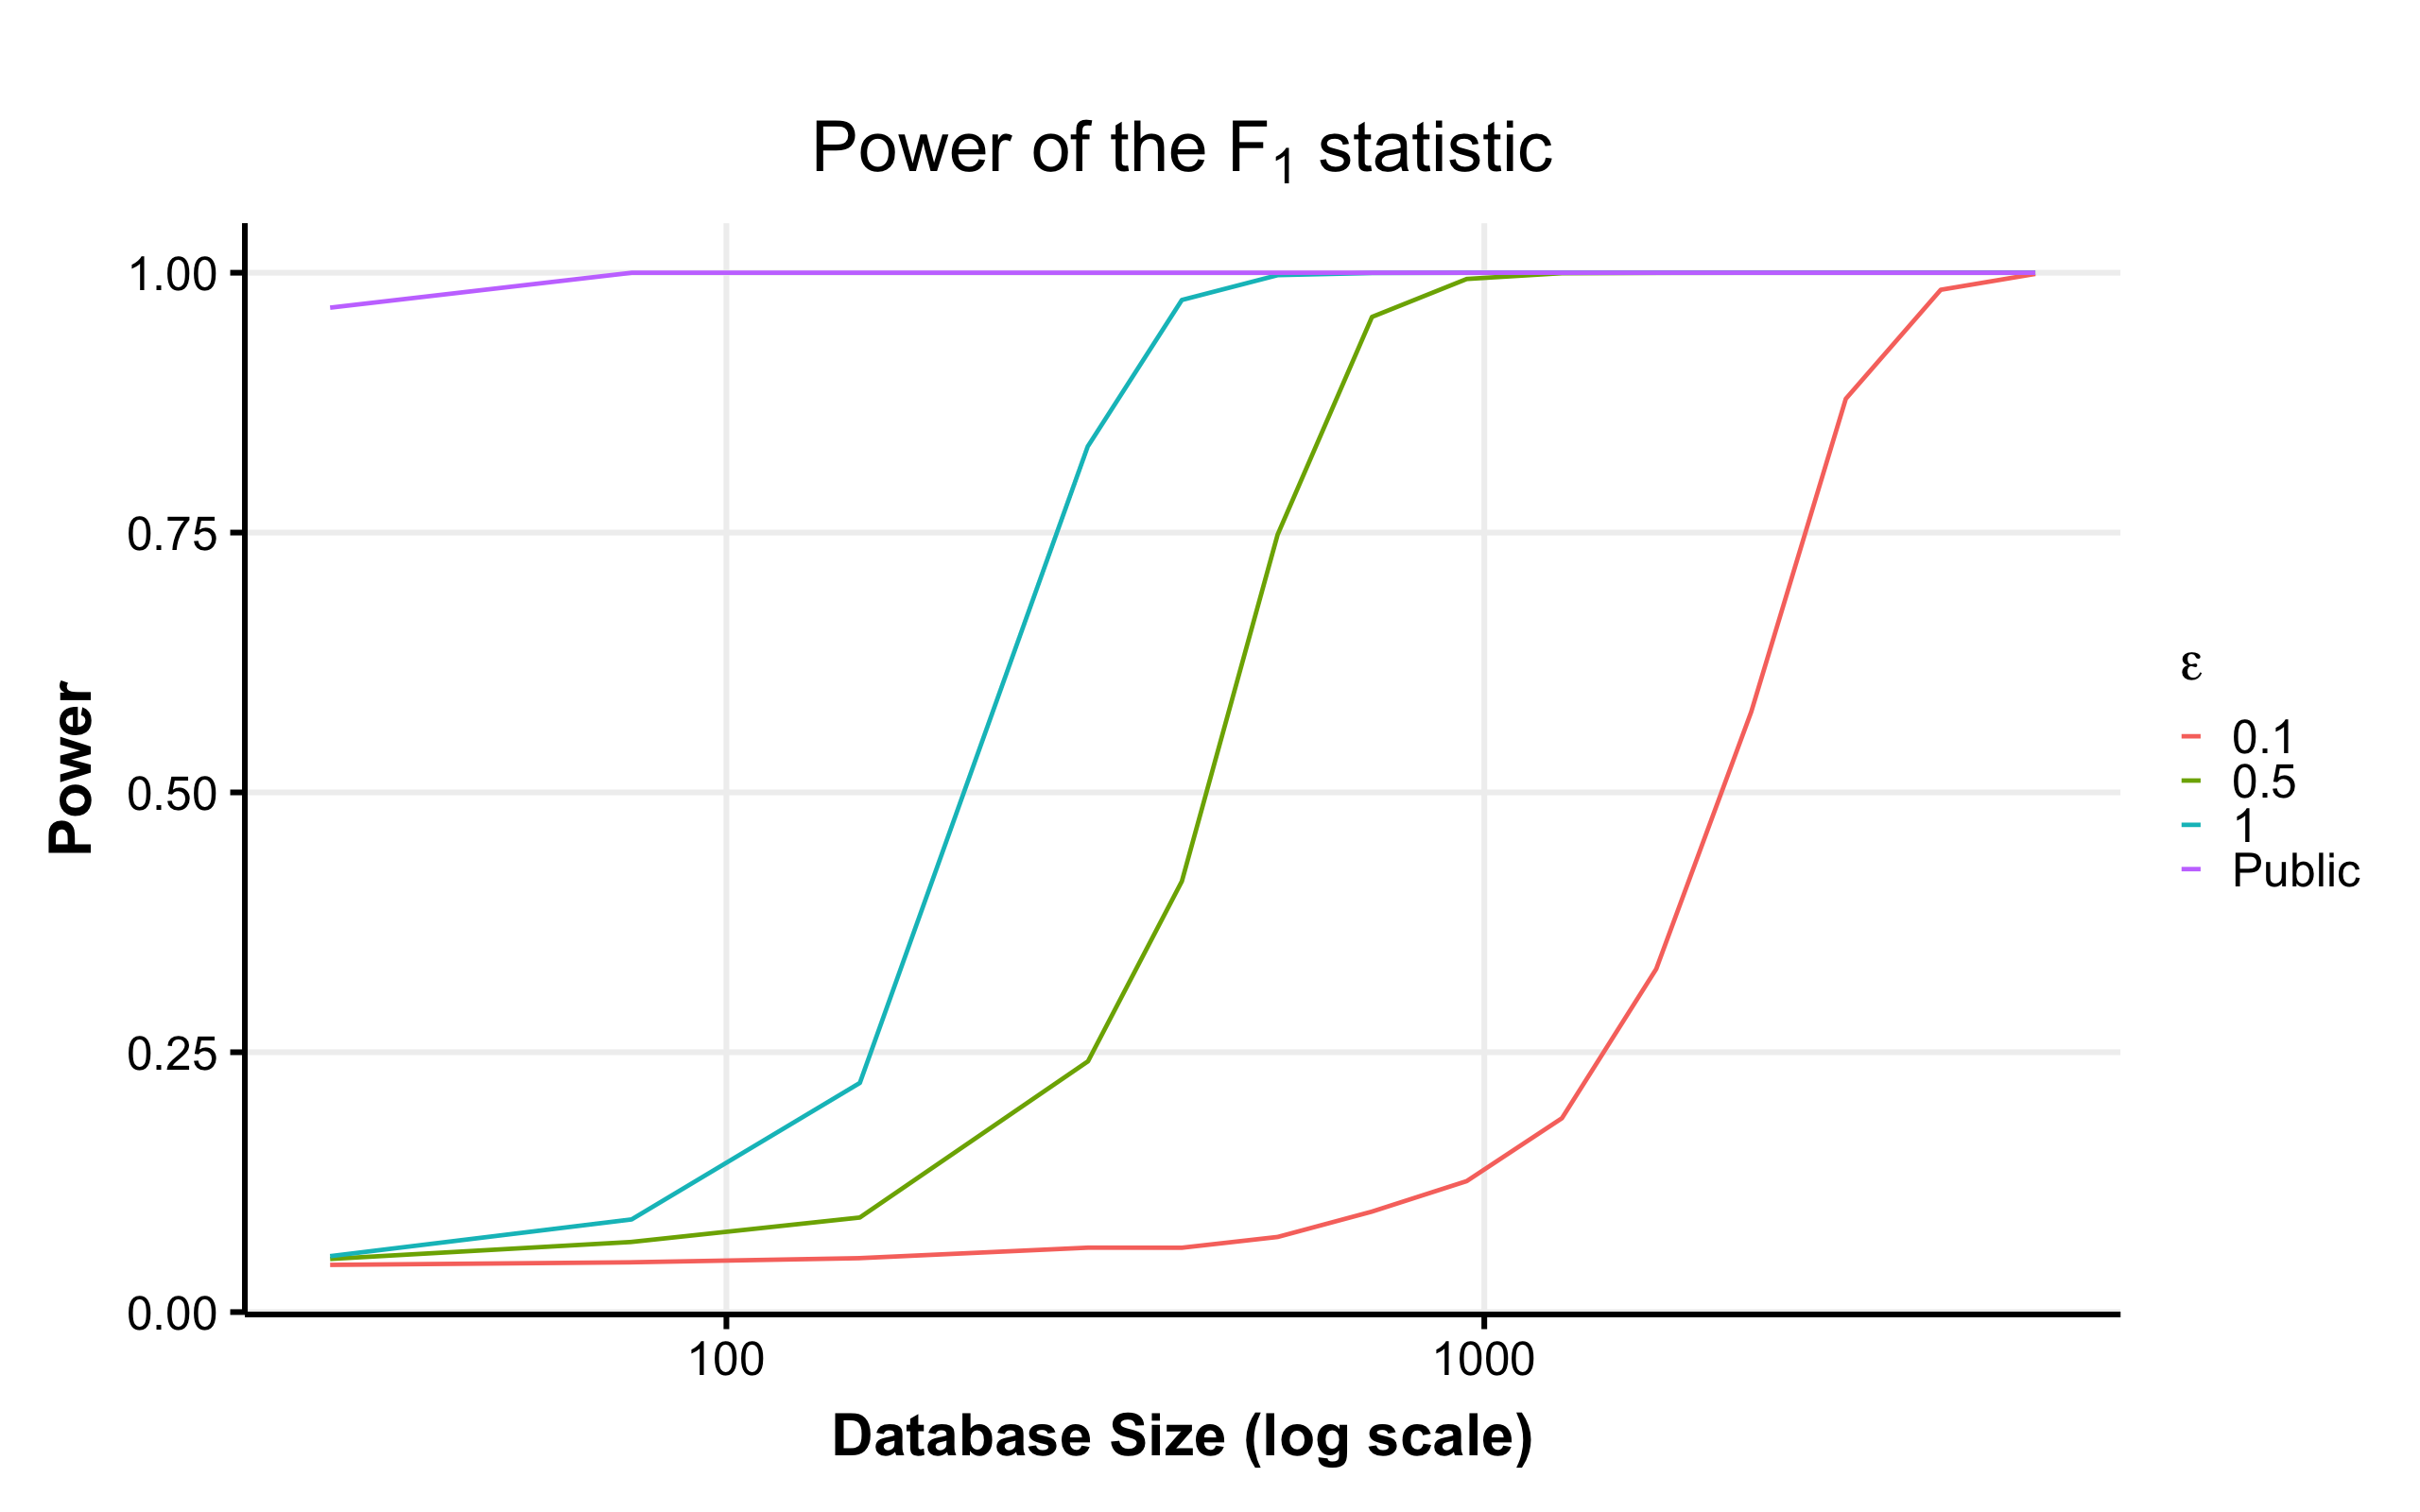
\includegraphics[width=.8\linewidth]{f1.png}
\caption{Power curves at varying privacy levels in a simulation setting where $k = 3$, $\sigma = .15$, and effect size: $1\sigma$.\label{Fig:f1}}
\end{figure}

Each point in a line of a power curve was computed from 10,000 simulations, each based on a synthetic database of a set sample size and a set effect size (distance between the group means).  We considered the effect $H_A$ where $\k=3$ groups, each distributed $\normal(0.35, 0.15),  \normal(0.5,0.15), \normal(0.65, 0.15)$ and equal group sizes, which was the same scenario as Campbell et al.~\cite{campbell2018diffprivanova}.
Each simulation starts with a draw from $H_A$ and computes a $p$-value as described in Algorithm~\ref{alg:pval}.

The most relevant comparison, however, is between the private $F_1$ statistic and the privatized version of the classical $F_2$ statistic proposed in Campbell et al., the only prior private version of ANOVA.  This comparison can be seen in Figure \ref{Fig:f1-vs-f2}, and the improvement is substantial.  For example, at $\epsilon = 1$, if one wanted to collect enough data to detect this effect with 80\% probability, one would need ~4500 observations if using the prior best test, whereas with the $F_1$ test presented here one would need only ~300 data points, a 15-fold reduction in the necessary amount of data.

\begin{figure}
\centering
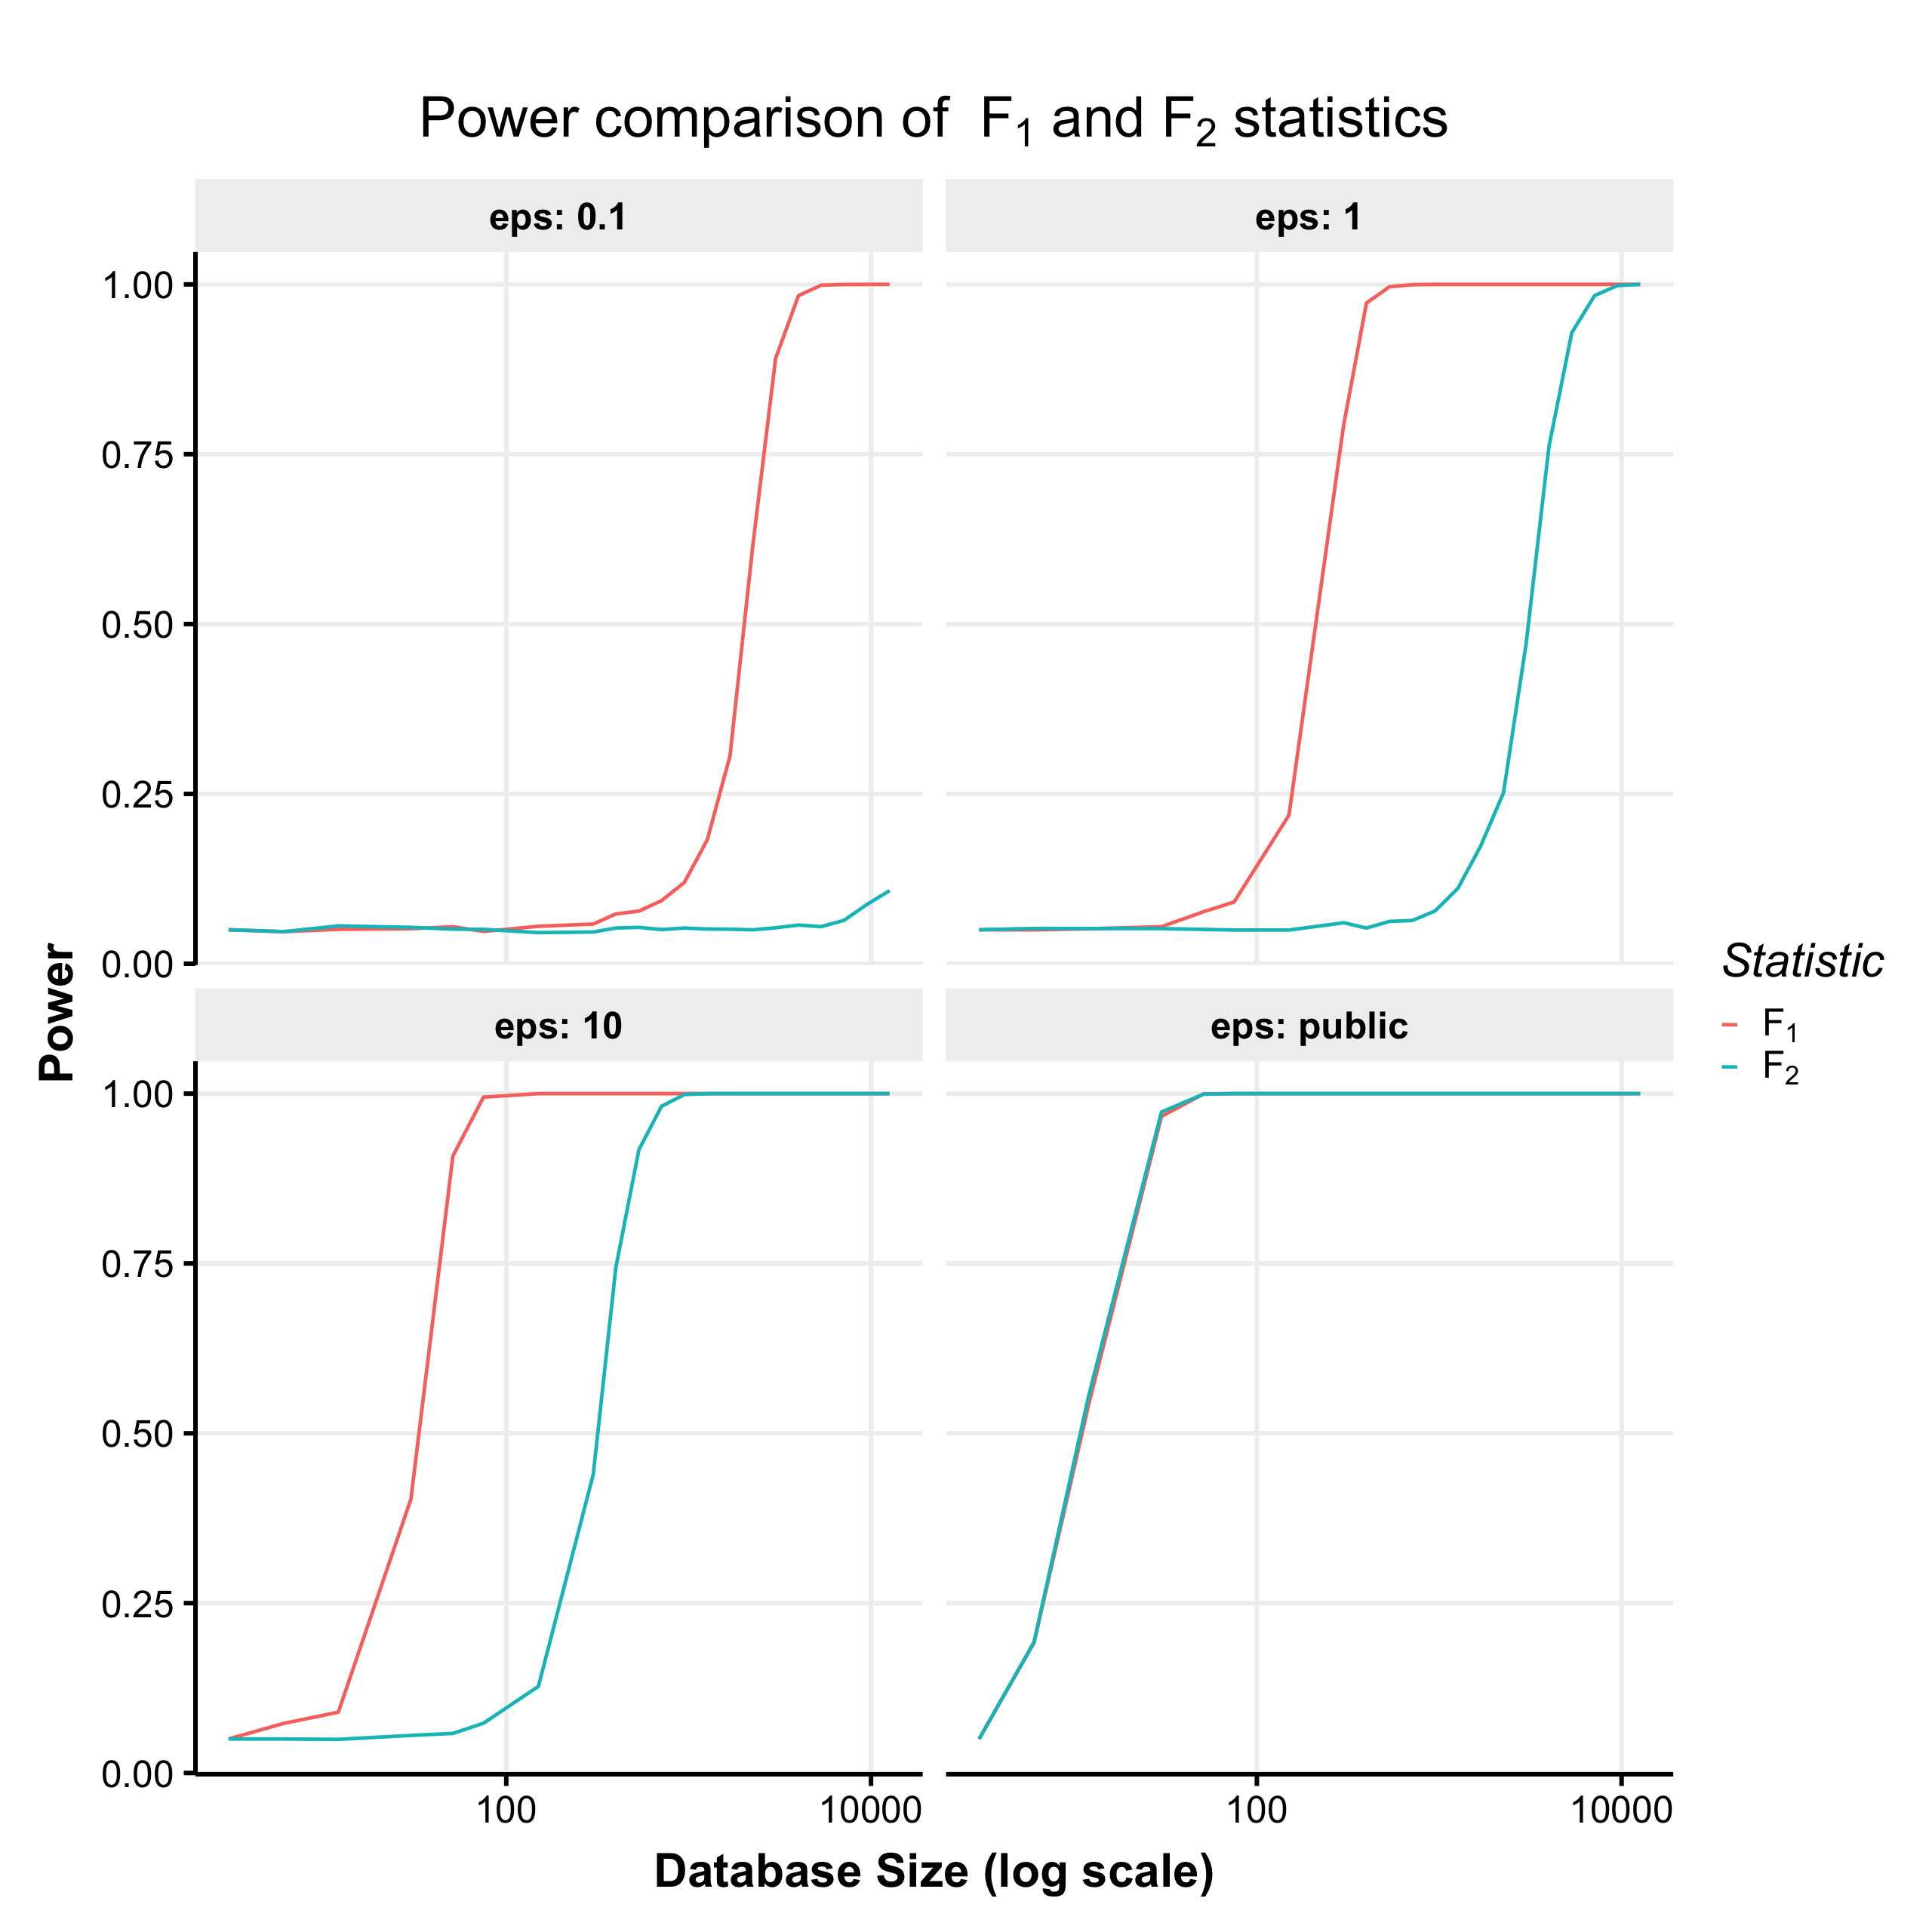
\includegraphics[width=.8\linewidth]{f1-vs-f2-quartet.png}
\caption{Comparison of the power of the new $F_1$-statistic and the prior state of the art test using $F_2$, for three values of $\epsilon$ and in the public setting.\label{Fig:f1-vs-f2}}
\end{figure}

Figure \ref{Fig:f1-vs-f2} also demonstrates the degree to which the $F_1$ is well-suited to the private setting; the greatest improvement in power occurs under high privacy ($\epsilon = 0.1$). As $\epsilon$ grows large, the difference between the two statistics shrinks. In the public setting, they are nearly indistinguishable, though the $F_2$ is narrowly more powerful at every database size.\footnote{This empirical result is consistent with theoretical results in the classical statistics literature that discuss conditions in which the $F_2$ is a most powerful test~\cite{cox1974theoretical}.}

The improvement in power is the greatest practical contribution of our work: the ability to conduct a private ANOVA with an order of magnitude less data than the existing approach. This improvement can be attributed to two key characteristics of our new test. The first and most important is the notion of measuring distance using the $L^1$ norm.  The second is the unequal apportionment of the privacy between the \sa and \se terms.

